\documentclass[10pt,a4paper,final]{article}
%
\usepackage[utf8x]{inputenc}
\usepackage{ucs}
\usepackage{amsmath}
\usepackage{geometry}
\usepackage{anysize} % Soporte para el comando \marginsize
\usepackage{graphicx}
\usepackage{listings}
\usepackage{amsfonts}
\usepackage{amssymb}
\usepackage[spanish]{babel}
%%%%%%%%%%%%%%%%%%%%%%%%%%%%%%%%%%%%%%%%%%%%%%%%%
%%%%%%%%%%%%%%%%%%%%%%%%%%%%%%%%%%%%%%%%%%%%%%%%%
%%%%%%%%%%%%%%%%%%%%%%%%%%%%%%%%%%%%%%%%%%%%%%%%%
\marginsize{2cm}{2cm}{1.5cm}{1.5cm}
%
\begin{document}
\title{Calculo de descensos en un campo de bombeo en medios porosos}
\author{Christian N. Pfarher, Juan Pablo Garbarino, Marina Castro\\
\textit{Trabajo práctico final de ``Métodos numéricos y simulación'', II-FICH-UNL.}}
\markboth{Método numérico y simulación: TRABAJO FINAL}{}
\date{\today}
\maketitle
%%%%%%%%%%%%%%%%%%%%%%%%%%%%%%%%%%%%%%%%%%%%%%%%%%%%%%%%%%%%%%%%%%%%%%%%%%%%%%%%%%%%%%%%%%%%%%%%%%
%%%%%%%%%%%%%%%%%%%%%%%%%%%%%%%%%%%%%%%%%%%%%%%%%%%%%%%%%%%%%%%%%%%%%%%%%%%%%%%%%%%%%%%%%%%%%%%%%%
%%%%%%%%%%%%%%%%%%%%%%%%%%%%%%%%%%%%%%%%%%%%%%%%%%%%%%%%%%%%%%%%%%%%%%%%%%%%%%%%%%%%%%%%%%%%%%%%%%
\newpage
\tableofcontents
%%%%%%%%%%%%%%%%%%%%%%%%%%%%%%%%%%%%%%%%%%%%%%%%%%%%%%%%%%%%%%%%%%%%%%%%%%%%%%%%%%%%%%%%%%%%%%%%%%
%%%%%%%%%%%%%%%%%%%%%%%%%%%%%%%%%%%%%%%%%%%%%%%%%%%%%%%%%%%%%%%%%%%%%%%%%%%%%%%%%%%%%%%%%%%%%%%%%%
%%%%%%%%%%%%%%%%%%%%%%%%%%%%%%%%%%%%%%%%%%%%%%%%%%%%%%%%%%%%%%%%%%%%%%%%%%%%%%%%%%%%%%%%%%%%%%%%%%
\newpage
%%%%%%%%%%%%%%%%%%%%%%%%%%%%%%%%%%%%%%%%%%%%%%%%%%%%%%%%%%%%%%%%%%%%%%%%%%%%%%%%%%%%%%%%%%%%%%%%%%
%%%%%%%%%%%%%%%%%%%%%%%%%%%%%%%%%%%%%%%%%%%%%%%%%%%%%%%%%%%%%%%%%%%%%%%%%%%%%%%%%%%%%%%%%%%%%%%%%%
%%%%%%%%%%%%%%%%%%%%%%%%%%%%%%%%%%%%%%%%%%%%%%%%%%%%%%%%%%%%%%%%%%%%%%%%%%%%%%%%%%%%%%%%%%%%%%%%%%
\section{Introducción}
El flujo subterráneo de agua es un componente importante de todos los sistemas hidráulicos. Tiene un papel central en el presupuesto de agua para uso doméstico, industrial y en agricultura. La administración del recurso implica tomar decisiones sobre donde perforar para extraer o inyectar y sobre las estrategias de control. También implica decisiones sobre la calidad del agua producida, lo que a su vez se relaciona con la disponibilidad del recurso.\\
Las reservas de agua subterránea como las \emph{napas} y los \emph{acuíferos} están formadas por la infiltración natural de agua de lluvia. Proveen el líquido a casas e industrias, a través de perforaciones individuales o de la explotación a gran escala por parte de empresas de servicios públicos.\\
Vamos a centrar nuestra atención en los acuíferos. Un acuífero es una formación geológica subterránea capaz de almacenar y rendir agua. El acuífero ocupa un dominio constituido por un medio poroso: tierra, arena, basaltos, granitos –usualmente fisurados– son todos ejemplos de medios porosos, que exhiben en común el estar constituidos por una matriz sólida y poros. Las condiciones geológicas e hidrológicas determinan su tipo y funcionamiento. Hay dos tipos de \emph{acuíferos}: los \emph{confinados} y los \emph{no confinados}. En el \emph{acuífero confinado}, el agua está atrapada entre las capas impermeables de la roca o entre grietas de la formación rocosa. Dicha agua podría encontrarse almacenada a presión. Si perforamos, el nivel de agua asciende hasta situarse en una determinada posición que coincide con el nivel de saturación del acuífero en el área de recarga.\\
Si la topografía es tal que la boca del pozo está por debajo del nivel del agua, el pozo es
surgente o artesiano; si no es así el nivel del agua ascenderá hasta el nivel correspondiente, pero no será surgente. El agua está sometida a una presión superior a la atmosférica y ocupa totalmente los poros o huecos de la formación geológica, saturándola totalmente. No existe zona no saturada. \\
Los acuíferos pueden estar cerca de la superficie terrestre, con estratos continuos formados por materiales de alta permeabilidad que se extienden desde la superficie del terreno hasta la base del acuífero. Este tipo de acuífero se conoce como un \emph{acuífero no confinado o libre}. La recarga de este acuífero se produce debido a una infiltración vertical a través de la zona no saturada. La recarga también se puede producir a través de flujo subterráneo lateral o desde estratos inferiores.\\
En un acuífero no confinado, el agua no está almacenada a presión por no estar encapsulada en la roca. Si se hiciera un pozo en él, el agua se tendría que bombear a la superficie.\\
En este trabajo trataremos el caso de un \emph{acuífero libre, homogéneo e isótropo}. 
Un medio \emph{homogéneo} es aquel que tiene las mismas propiedades en todas las posiciones. Esto significa que la porosidad y otros parámetros son similares en cualquier posición dentro de la unidad geológica.\\
En un medio poroso compuesto de esferas del mismo diámetro, agrupadas uniformemente, la geometría de los huecos vacíos es la misma en cualquier dirección. De esta manera, la permeabilidad del medio es la misma en cualquier dirección, y el medio se denomina \emph{isotrópico}.
El campo consta de dos pozos de bombeo de agua que funcionan un cierto período de tiempo extrayendo un caudal de agua.
Para la realización del trabajo se utilizó el software de pre y pos proceso GiD \footnote{http://gid.cimne.upc.es/}. Mediante el mismo, se utilizó el \emph{módulo de pre-proceso} para la carga de los datos del problema, mientras que para la simulación se utilizó Tdyn \footnote{es un entorno tridimensional de análisis fluidodinámico (CFD) y multifísica basado en el método de los elementos finitos estabilizado}(\emph{módulo de post-proceso}).
%%%%%%%%%%%%%%%%%%%%%%%%%%%%%%%%%%%%%%%%%%%%%%%%%%%%%%%%%%%%%%%%%%%%%%%%%%%%%%%%%%%%%%%%%%%%%%%%%%
%%%%%%%%%%%%%%%%%%%%%%%%%%%%%%%%%%%%%%%%%%%%%%%%%%%%%%%%%%%%%%%%%%%%%%%%%%%%%%%%%%%%%%%%%%%%%%%%%%
%%%%%%%%%%%%%%%%%%%%%%%%%%%%%%%%%%%%%%%%%%%%%%%%%%%%%%%%%%%%%%%%%%%%%%%%%%%%%%%%%%%%%%%%%%%%%%%%%%
\section{Objetivos}
El objetivo de este trabajo, consiste en la simulación de lineas de corrientes y equipotenciales en un campo de bombeo (medio poroso) con 2 bombas de extracción de agua en un acuífero libre (no confinado), homogéneo e isótropo. \begin{LARGE}
ver bien que vamos a poner como objetivos
\end{LARGE}

%%%%%%%%%%%%%%%%%%%%%%%%%%%%%%%%%%%%%%%%%%%%%%%%%%%%%%%%%%%%%%%%%%%%%%%%%%%%%%%%%%%%%%%%%%%%%%%%%%
%%%%%%%%%%%%%%%%%%%%%%%%%%%%%%%%%%%%%%%%%%%%%%%%%%%%%%%%%%%%%%%%%%%%%%%%%%%%%%%%%%%%%%%%%%%%%%%%%%
%%%%%%%%%%%%%%%%%%%%%%%%%%%%%%%%%%%%%%%%%%%%%%%%%%%%%%%%%%%%%%%%%%%%%%%%%%%%%%%%%%%%%%%%%%%%%%%%%%
\section{Base Teórica}
%%%%%%%%%%%%%%%%%%%%%%%%%%%%%%%%%%%%%%%%%%%%%%%%%%%%%%%%%%%%%%%%%%%%%%%%%%%%%%%%%%%%%%%%%%%%%%%%%%%
\subsection{Modelo matemático}
Para la resolución del problema utilizamos \emph{Tdyn}, el cual está basado en la solución numérica de las ecuaciones de \emph{Navier-Stokes} empleando el \emph{FEM}.
\emph{Tdyn} resuelve las ecuaciones de Navier-Stokes en tres dimensiones para un fluido incompresible o ligeramente compresible de un dominio $\Omega$ dado y un intervalo de tiempo $(0,t):$
\begin{eqnarray}
\rho \left(\frac{\partial u}{\partial t}+\left( u \bullet  \nabla \right)u \right)+ \nabla p - \nabla \bullet(\mu \nabla u) &=& \rho f~ \mbox{ en  }\Omega \times (0,t)\\
\nabla \bullet u&=&0 ~ \mbox{ en  } \Omega \times (0,t)
\end{eqnarray}
donde $u = u(x,t)$ denota el vector velocidad, $p=p(x,t)$ el campo de presiones, $\rho$ la densidad (constante), $\mu$ la viscosidad dinámica del fluido y la $f$ la aceleración volumétrica.\\
Las ecuaciones de arriba necesitan ser combinadas con las siguientes condiciones de borde:
\begin{eqnarray}
u &=& u_c \mbox{ en  } \Gamma_D \times (0,t);\\
p &=& p_c \mbox{ en  } \Gamma_P \times (0,t);\\
n \cdot \sigma \cdot g_1=0 \mbox{, } n \cdot \sigma \cdot g_2=0~ \mbox{, } n \cdot u&=&u_M \mbox{ en  } \Gamma_M \times (0,t);\\
u(x,0)&=&u_0(x) \mbox{ en  } \Omega_D \times \lbrace 0 \rbrace ;\\
p(x,0)&=&p_0(x) \mbox{ en  } \Omega_D \times \lbrace 0 \rbrace ;
\end{eqnarray}
En las ecuaciones de arriba, $\Gamma = \partial \Omega$ denota la forntera del dominio $\Omega$, siendo $n$ el vector normal unitario y $g_1$, $g_2$ los vectores tangentes de la frontera $\partial \Omega$, $u_c$ es el campo de velocidad sobre $\Gamma_D$, $p_c$ la presión sobre $\Gamma_P$, $\sigma$ es el campo de tensiones, $u_M$ el valor de la velocidad normal y $u_0$, $p_0$ los campos de velocidad y presión iniciales. La unión de $\Gamma_D$, $\Gamma_P$ y $\Gamma_M$ debe ser $\Gamma$; la intersección entre ellos es el conjunto vacío, ya que un punto de la frontera puede ser parte de un único tipo de superficie, a menos que forme parte del borde entre dos de ellas.

La discretización espacial de las ecuaciones de \emph{Navier - Stokes} es realizada mediante el método de elementos finitos, mientras que para la discretización en el tiempo debe considerarse un algoritmo iterativo tal como el \emph{Método de pasos fraccionarios (Fractional Step Method) de dos pasos (implícito)}.

También hay que aclarar que no se utiliza un modelo te turbulencia (como lo es el de Smagorinsky) ya que se está en presencia de un flujo lento.
%%%%%%%%%%%%%%%%%%%%%%%%%%%%%%%%%%%%%%%%%%%%%%%%%%%%%%%%%%%%%%%%%%%%%%%%%%%%%%%%%%%%%%%%%%%%%%%%%%
\subsection{Ley de Darcy}
La \emph{Ley de Darcy} expresa que el flujo de agua en un medio poroso, homogéneo e isotrópico es proporcional 
a la conductividad del medio poroso o conductividad hidráulica $K$ y a una fuerza conductora o gradiente hidráulico $i$.
\\
La expresión matemática de la \emph{Ley de Darcy} viene dada por la ecuación (\ref{darcy_formula})
\begin{eqnarray}
Q&=&K \frac{h_3 - h_4}{L} A = K \cdot i \cdot A \label{darcy_formula}
\end{eqnarray}
donde:
\begin{itemize}
	\item[$Q=$] gasto, descarga o caudal en $m^3/s$,
	\item[$L=$] longitud en metros de la muestra,
	\item[$K=$] una constante, actualmente conocida como coeficiente de permeabilidad de Darcy, variable en función del material de la muestra, en $m/s$,
	\item[$A=$] área de la sección transversal de la muestra, en $m^2$,
	\item[$h_3=$] altura, sobre el plano de referencia que alcanza el agua en un tubo colocado a la entrada de la capa filtrante,
	\item[$h_4=$] altura, sobre el plano de referencia que alcanza el agua en un tubo colocado a la salida de la capa filtrante,
	\item[$i=$] $\frac{h_3 - h_4}{L}=$ el gradiente hidráulico.
\end{itemize}
%
\begin{figure}[tbhp]
\centerline{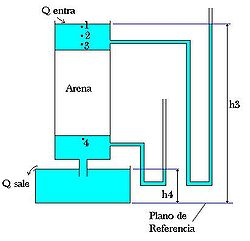
\includegraphics[scale=0.6]{img/darcy_grafica}}
\caption{Ley de Darcy}
\label{graf_leydarcy}
\end{figure}
%
La ley de Darcy es válida para todo suelo donde el flujo sea laminar: arenas finas a medias, arenas gruesas bien graduadas, arcillas y limos. Entre sus limitaciones, es posible afirmar que la constante de proporcionalidad $K$ no es propia del medio poroso, sino que depende de las características del fluido (peso específico y viscosidad cinemática). 
El factor $K$ se puede descomponer como se puede ver en (\ref{k_descompuesto}) 
\begin{eqnarray}
	K&=& k \cdot x \cdot \gamma \cdot \mu \label{k_descompuesto}
\end{eqnarray}
donde: 
\begin{itemize}
	\item[$K=$] permeabilidad de Darcy o conductividad hidraúlica,
	\item[$k=$] permeabilidad intrínseca (depende solo del medio poroso)
	\item[$\gamma=$] peso específico del fluido
	\item[$\mu=$] viscosidad dinámica del fluido
\end{itemize}
Esta cuestión es fundamental en geología del petróleo, donde se estudian fluidos de diferentes características. En el caso del agua, la salinidad apenas hace variar el peso específico no la viscosidad.
Solamente habría que considerar la variación de la viscosidad con la temperatura, que se duplica entre 5 y 35 º C, con lo que se duplicaría la permeabilidad de Darcy y también el caudal circulante por la sección considerada del medio poroso. Afortunadamente, las aguas subterráneas presentan mínimas diferencias de temperatura a lo largo del año en un mismo acuífero.
Por tanto, aunque sabemos que $K$ depende tanto del medio como del propio fluido, como la parte que depende del fluido normalmente es despreciable, a efectos prácticos asumimos que la $K$ de Darcy, o \emph{conductividad hidráulica} es una característica del medio poroso.
\\
En algunas circunstancias, la relación entre el caudal y el gradiente hidráulico no es lineal.
Esto puede suceder cuando el valor de $K$ es muy bajo o cuando las velocidades del flujo son muy altas.
En el primer caso, por ejemplo, calculando el flujo a través de una formación arcillosa, el caudal que obtendríamos aplicando la Ley de Darcy sería bajísimo, pero en la realidad, si no se aplican unos gradientes muy elevados, el agua no llega a circular, el caudal es 0.
En el segundo caso, si el agua circula a gran velocidad, el caudal es directamente proporcional a la sección y al gradiente, pero no linealmente proporcional.
En el flujo subterráneo las velocidades son muy lentas y prácticamente siempre la relación es lineal, salvo en las proximidades de captaciones bombeando en ciertas condiciones.
%%%%%%%%%%%%%%%%%%%%%%%%%%%%%%%%%%%%%%%%%%%%%%%%%%%%%%%%%%%%%%%%%%%%%%%%%%%%%%%%%%%%%%%%%%%%%%%%%%
%%%%%%%%%%%%%%%%%%%%%%%%%%%%%%%%%%%%%%%%%%%%%%%%%%%%%%%%%%%%%%%%%%%%%%%%%%%%%%%%%%%%%%%%%%%%%%%%%%
%%%%%%%%%%%%%%%%%%%%%%%%%%%%%%%%%%%%%%%%%%%%%%%%%%%%%%%%%%%%%%%%%%%%%%%%%%%%%%%%%%%%%%%%%%%%%%%%%%
\section{Desarrollo}
%%%%%%%%%%%%%%%%%%%%%%%%%%%%%%%%%%%%%%%%%%%%%%%%%%%%%%%%%%%%%%%%%%%%%%%%%%%%%%%%%%%%%%%%%%%%%%%%%%
\subsection{Datos del problema}
\label{datos_problema}
Los datos que se pudieron obtener del problema son:
\begin{itemize}
	\item Discretización del área a modelar:	
	\begin{itemize}
		\item Dominio: $x=1000 ~\left[m\right]$, $y=1000 ~\left[m\right]$
		\item Acuífero libre, homogéneo e isótropo $(K_{xx} = K_{yy} = K_{zz})$
		\item Espesor del acuífero: $20 ~\left[m\right]$
	\end{itemize}
	%
	\item Ubicación de los Pozos de bombeo:
	\begin{itemize}
		\item Pozo Bombeo 1: $x=150~~\left[m\right]$, $y=650 ~~\left[m\right]$
		\item Pozo Bombeo 2: $x=750~~\left[m\right]$, $y=250 ~~\left[m\right]$
	\end{itemize}
	%
	\item Caudal de bombeo:
	\begin{itemize}
		\item Pozo Bombeo 1: $60~\left[\frac{m³}{h}\right]$
		\item Pozo Bombeo 2: $40~\left[\frac{m³}{h}\right]$
	\end{itemize}
	\item Diámetro del pozo: $0.5 [m]$* \begin{Large} esto no era dato! pero los calculso lo hicimos con este valor \end{Large}
	\item Filtro: Tramo filtrante de longitud $15~m.$
	\item Transmisividad: $600~\left[\frac{m^2}{d}\right]$\\
\begin{LARGE}
Coef de trasmisividad: cuanto mas chiquito es mas lento se mueve el agua en el suelo.ver!! \\
\end{LARGE}	
	\item Coeficiente de almacenamiento: $5*10⁻²$ \begin{LARGE}
	creo que este no lo usamos... ver
	\end{LARGE}
	\item Porosidad efectiva: $5*10⁻²$
\end{itemize}
\begin{Large}
También hay que aclarar que nos encontramos en presencia de suelo saturado, esto es.....ver!\\
\end{Large}

%%%%%%%%%%%%%%%%%%%%%%%%%%%%%%%%%%%%
\subsubsection{Cálculo de la velocidad de extracción de agua a partir del caudal}
Se procedió a convertir las unidades de los datos del problema (Caudal de extracción de los pozos a velocidad) para poder ingresarlas en el software de simulación.
En dinámica de fluidos, \emph{caudal} es la cantidad de fluido que avanza en una unidad de tiempo. Se denomina también ``Caudal volumétrico" o ``Indice de flujo fluido". El cálculo del caudal de agua viene expresado por:
\begin{equation}
Q=V \cdot S
\label{caudal}
\end{equation}
donde en la ecuación (\ref{caudal}) $Q$ es el caudal, $V$ es la velocidad y $S$ es la sección de la tubería
%
\begin{itemize}
\item Pozo de Bombeo 1: a partir de la ec. (\ref{caudal}) y dado que se conoce el caudal del pozo de bombeo 1 $Q_1=60 \left[\frac{m³}{h} \right]$ se puede calcular la velocidad de extracción $V_1$ como:\\
\begin{eqnarray*}
Q_1&=&V_1 \cdot S_1 \\
Q_1/S_1&=&V_1 \\
\frac{60 \left[\frac{m^3}{h}\right]}{\pi \cdot r^2} &=&V_1~~\textrm{donde $r$ es el radio de la tubería}\\
\mbox {dado que $r=0.25 \left[m\right]$ y reemplazando}\\
\frac{1 \left[h\right]}{3600 \left[s\right]}\cdot\frac{60 \left[\frac{m^3}{h}\right]}{\pi \cdot 0.25^2 [m^2]}&=&V_1 \\
0.084883 \left[\frac{m}{s}\right]& = & V_1\\
0.085 \left[\frac{m}{s}\right]&\approx& V_1\\
\end{eqnarray*}
\item Pozo de Bombeo 2: procediendo de la misma manera escrita arriba y con el caudal del pozo de bombeo 2 $Q_2=40 \left[\frac{m³}{h} \right]$ se puede calcular la velocidad de extracción $V_2$ como:\\
\begin{eqnarray*}
Q_2&=&V_2 \cdot S_2 \\
Q_2/S_2&=&V_2 \\
\frac{40 \left[\frac{m^3}{h}\right]}{\pi \cdot r^2} &=&V_1~~\textrm{donde $r$ es el radio de la tubería}\\
\mbox {dado que $r=0.25 \left[m\right]$ y reemplazando}\\
\frac{1 \left[h\right]}{3600 \left[s\right]}\cdot\frac{40 \left[\frac{m^3}{h}\right]}{\pi \cdot 0.25^2 [m^2]}&=&V_2 \\
0.056588 \left[\frac{m}{s}\right]& = & V_2\\
0.057 \left[\frac{m}{s}\right]&\approx& V_2\\
\end{eqnarray*}
\end{itemize}
%%%%%%%%%%%%%%%%%%%%%%%%%%%%%%%%%%%%%%%%%%%%%%%%%%%%%%%%%%%%%%%%%%%%%%%%%%%%%%%%%%%%%%%%%%%%%%%%%%%
\subsection{Definición de Geometría}
Para la geometría en tres dimensiones se tiene los siguientes datos:
En las figuras \ref{cotas_superiores_generalesXY}, \ref{cotas_superiores_detallesXY} y \ref{cotas_grales_YZ} se pueden observar
las dimensiones de las geometrías según los datos del problema. Hay que aclarar aquí que el cuadrado de $300~m.~x~300~m.$ que se visualiza
en la figura \ref{cotas_superiores_detallesXY} como el rectángulo de $400~m.~x~300~m.$ en la misma figura, solo fueron dibujados con el
objetivo, de a posteriori, realizar un refinamiento del dominio en la zona que más interesa visualizar.\\
También, se debe aclarar, que tanto el \emph{tramo filtrante}, el \emph{espesor del acuífero} y el \emph{diámetro de los pozos} descriptos en la sección \ref{datos_problema} fueron redimensionados con el objetivo de tener una  mejor visualización de los resultados, quedando con las siguientes dimensiones:
\begin{itemize}
		\item Espesor del acuífero(amplificado por un factor 10): $200 ~\left[m\right]$*
		\item Tramo filtrante de longitud (amplificado por un factor 10): $150~m.$*
		\item Diámetro del pozo (amplificado por un factor 40): $20 [m]$*
		\begin{Large}
		que vamos a poner al final? que la simulacion se hizo en un radio de 20 m? o que la redimensiones fue echa con ese objetivo? me parece que esto esta mal pero bueno.. ver que haceR!
		\end{Large}
\end{itemize}
A continuación se presentan los datos de los elementos que forman la geometría:
\begin{itemize}
\item Número de puntos: 33
\item Número de lineas: 52
\item Número de superficies: 28
\item Número de volumenes: 3
\end{itemize}

\begin{figure}[tbhp]
\centerline{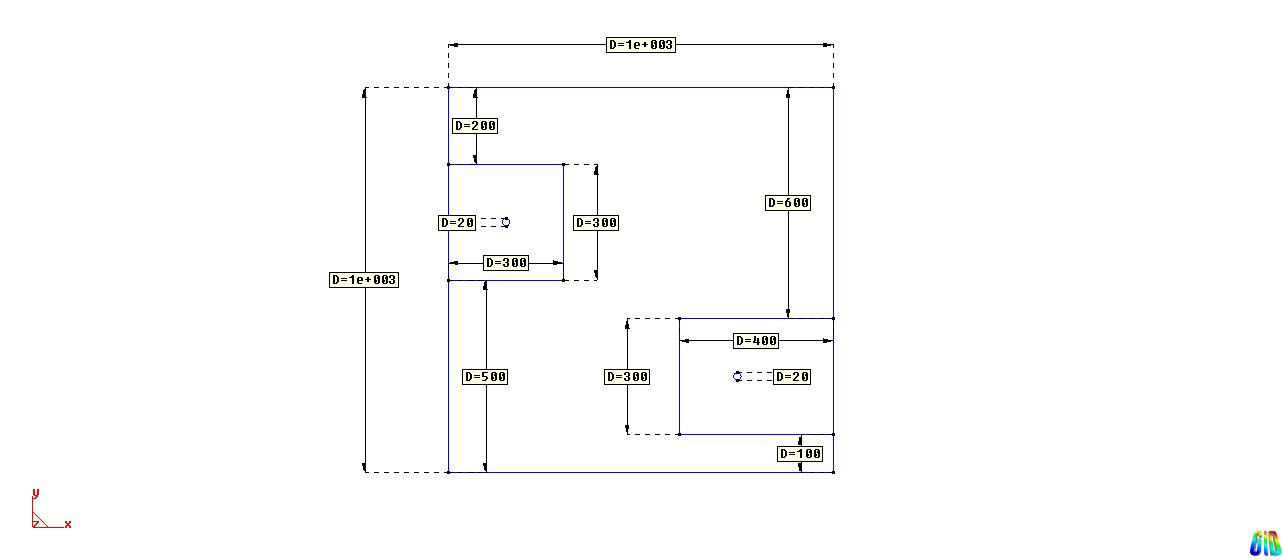
\includegraphics[scale=0.75]{img/cotas_superiores_generalesXY}}
\caption{Vista General de las cotas en el Plano XY}
\label{cotas_superiores_generalesXY}
\end{figure}

%
\begin{figure}[tbhp]
\centerline{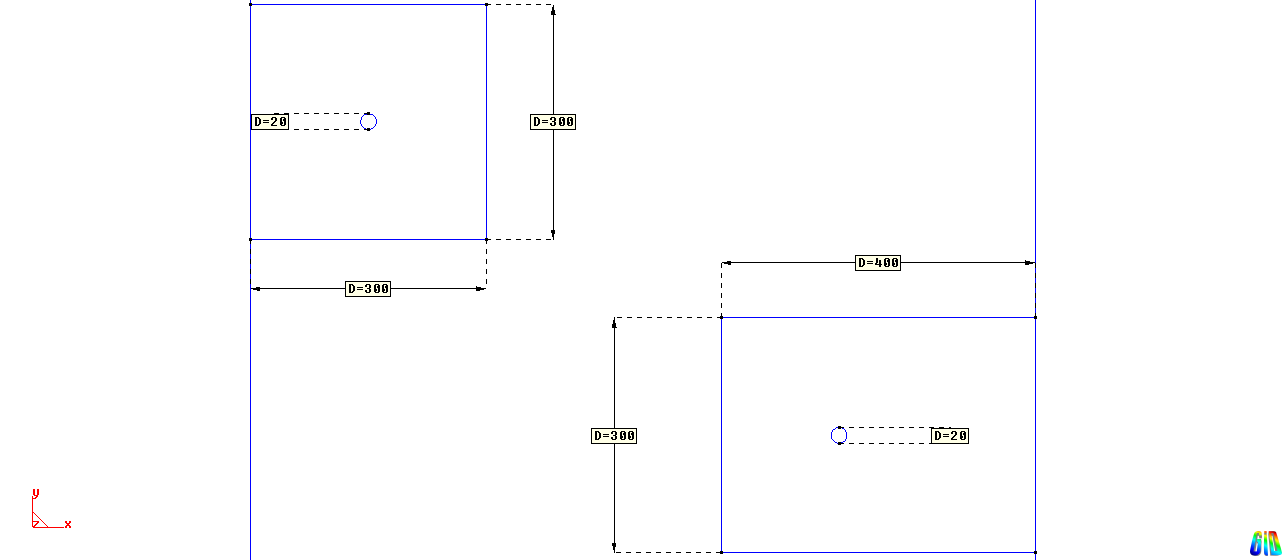
\includegraphics[scale=0.6]{img/cotas_superiores_detallesXY}}
\caption{Vista en detalle (pozos) de las cotas en el Plano XY}
\label{cotas_superiores_detallesXY}
\end{figure}
%

%
\begin{figure}[tbhp]
\centerline{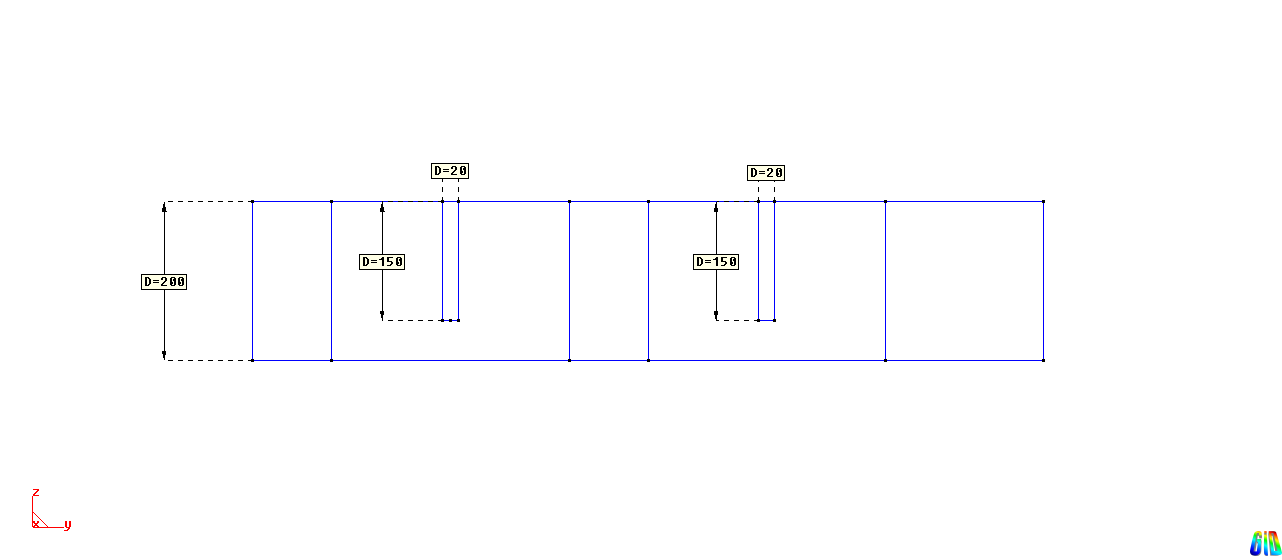
\includegraphics[scale=0.6]{img/cotas_grales_YZ}}
\caption{Vista en de las cotas en el plano YZ}
\label{cotas_grales_YZ}
\end{figure}
%
En la figura \ref{superficies_y_volumenes} se pueden observar las generaciones de las superficies (color magenta) y volúmenes (color cyan)
de la geometría.
%
\begin{figure}[tbhp]
\centerline{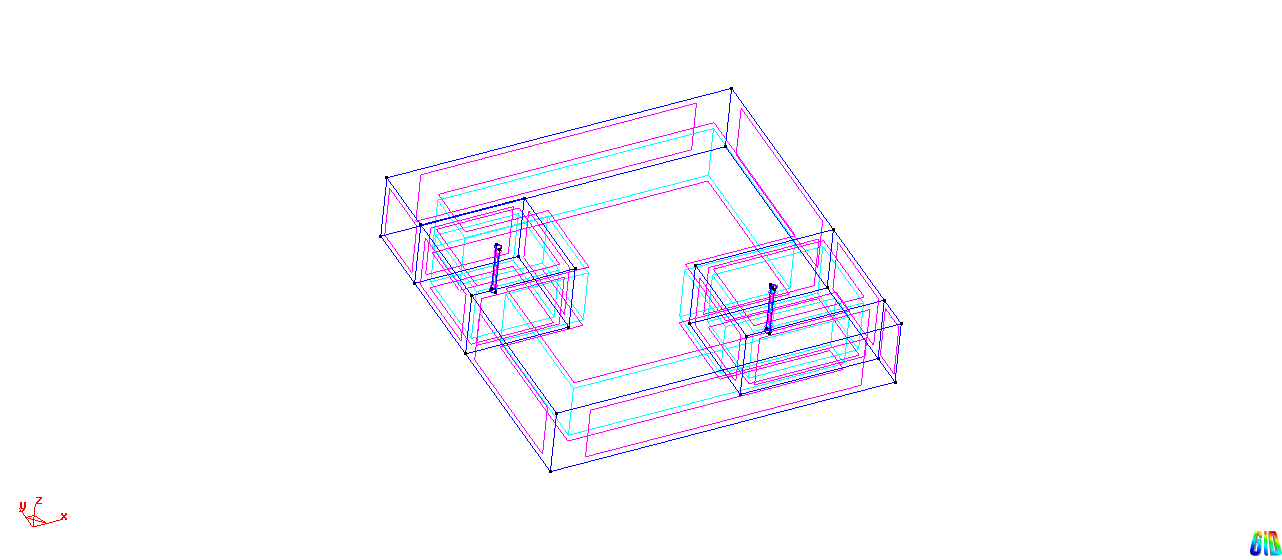
\includegraphics[scale=0.75]{img/superficies_y_volumenes}}
\caption{Superficies y Volúmenes de la Geometría}
\label{superficies_y_volumenes}
\end{figure}
%
%%%%%%%%%%%%%%%%%%%%%%%%%%%%%%%%%%%%%%%%%%%%%%%%%%%%%%%%%%%%%%%%%%%%%%%%%%%%%%%%%%%%%%%%%%%%%%%%%%%
\subsection{Propiedades del medio y de los materiales}
A partir de los datos del problema se tuvieron que realizar conversiones de unidades y el cálculo de diferentes valores para ser ingresados en el programa GID para definir los parámetros del modelo.
%%%%%%%%%%%%%%%%%%%%%%%%%%%%%%
\subsubsection{Material Suelo}
En la pestaña ransol de la ventana de materiales de fluidos para el material suelo de  se introdujeron los siguientes valores:
\begin{itemize}
\item Modelo de Fluido: flujo incompresible (la densidad del fluido permanece constante con el tiempo $\rho = cte.$)
\item Densidad: $999.7~Kg/m^3$ (agua a $10° C$) \footnote{ según datos obtenidos de Tabla-libro ...}
\item Viscosidad: $0.001307~Pa.s$ (agua a $10° C$)\footnote{ según datos obtenidos de Tabla-libro ...}
\item Resistencia de la Ley de Darcy:
quizas explicar que corno y como se haya este coeficiente de 0.0000017 y que representa la ley de darcy.. porosidad del suelo...\\
	k = conductividad 1\/ m \^2 o 1 \/ darcy\\
silvina: Ley de resistencia de darcy: es la ley que habla de la velocidad que tiene el agua para moverse dentro del medio poroso. Hay 6 valores porque este coef puede ser homogeneo en todo el suelo, esto se llama suelo isotropico, es el que tiene el mismo coef de trasmisividad en todos los sentidos: x,y,z. Cuando el suelo tiene distinto coef se usa toda la matriz que es lo real y lo normal. A los fines del cálculo lo usamos como isotropico, entonces solo completamos la diag principal y con el mismo valor (hay que ver el tema de la unidad, porque esta distinta a los datos). 
\begin{equation}
\begin{pmatrix}{}
0.0000017 & 0.0 & 0.0 \\ 
0.0 & 0.0000017 & 0.0 \\ 
0.0 & 0.0 & 0.0000017
\end{pmatrix} [1/m²]
\label{matrizdarcys}
\end{equation}
Debido a que se está en presencia de un acuífero isótropo, en (\ref{matrizdarcys}) se puede observar que sólo la diagonal principal de la matriz presenta valores diferentes de cero.
\end{itemize}
En la figura \ref{datos_materiales_suelo_vista} se puede observar la asignación del material definido a la parte del dominio correspondiente.

\begin{figure}[tbhp]
\centerline{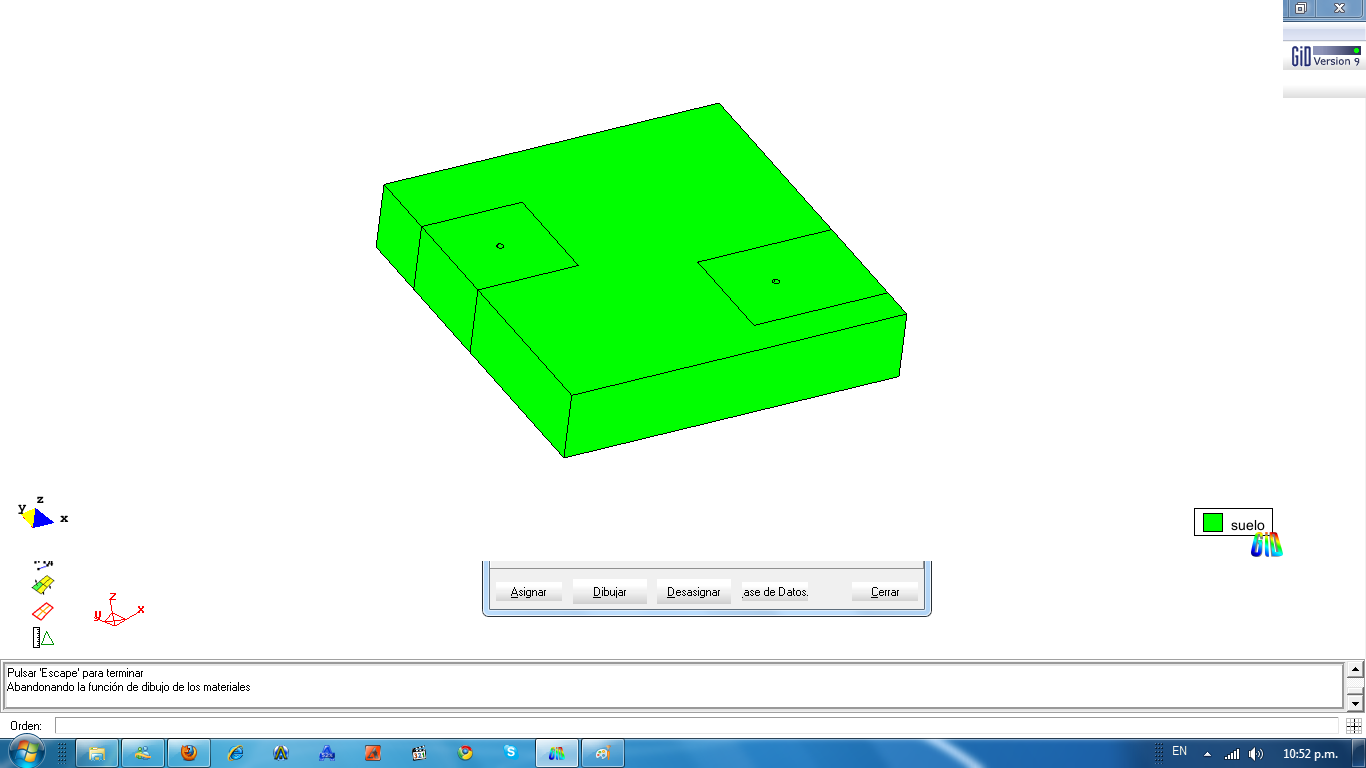
\includegraphics[scale=0.75]{img/datos_materiales_suelo_vista}}
\caption{Material Suelo asignado a la geometría}
\label{datos_materiales_suelo_vista}
\end{figure}
%%%%%%%%%%%%%%%%%%%%%%%%%%%%%%%
\subsubsection{Material Wall o Pared}
En la ventana de contornos fluidos se asigno a las paredes de ambos pozos el contorno definido por defecto Wall. El tipo de contorno seleccionado fue el \emph{V fixWall} con el ángulo por defecto de $60°$. Este es el modelo elegido en Tdyn para simular el comportamiento del flujo en las paredes del dominio. Básicamente, impone que la velocidad en las superficies asignadas será nula, modelando así la pared del pozo por la que no existe penetración de agua hacia el interior del pozo. En la figura \ref{datos_contornos_fluidos_vista} se puede observar el material asignado a ambos pozos.
\begin{figure}[tbhp]
\centerline{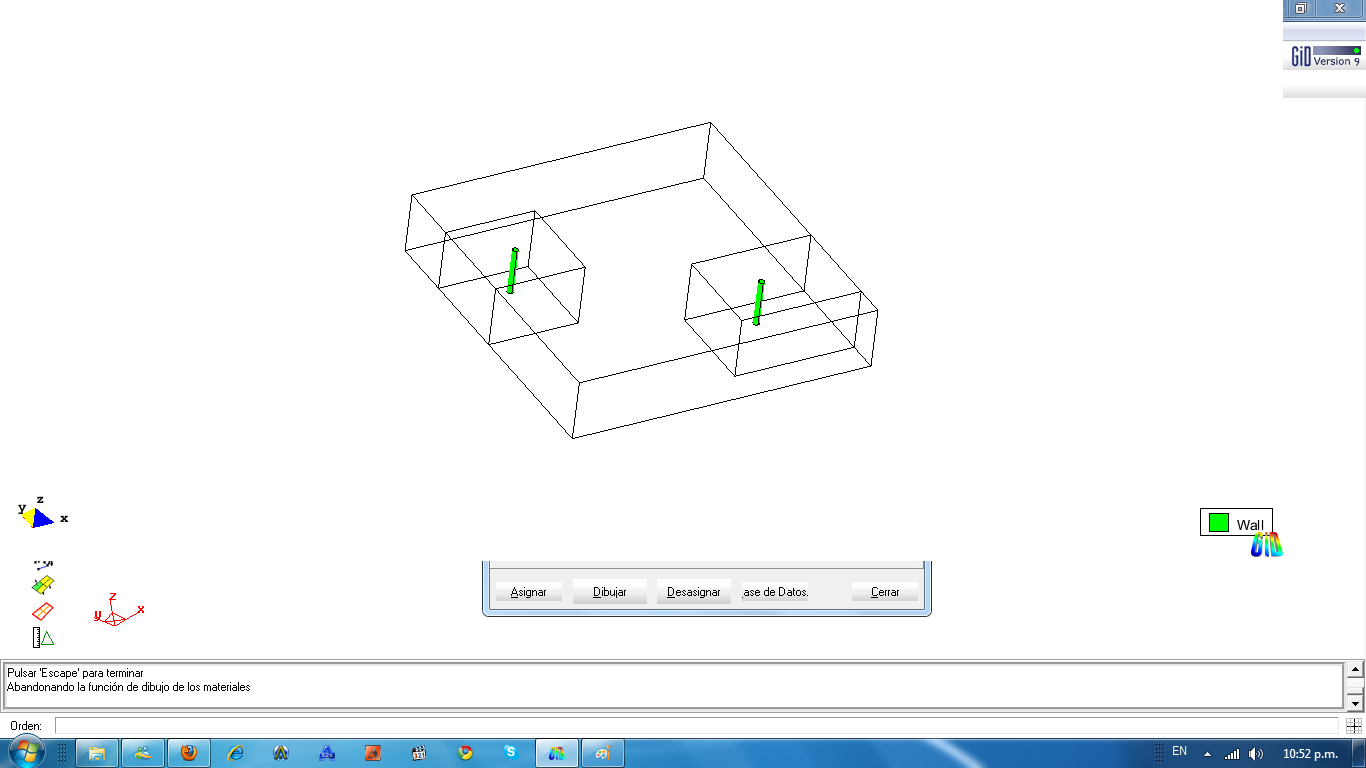
\includegraphics[scale=0.75]{img/datos_contornos_fluidos_vista}}
\caption{Material Wall o Pared asignado a la geometría}
\label{datos_contornos_fluidos_vista}
\end{figure}
%%%%%%%%%%%%%%%%%%%%%%%%%%%%%%%%%%%%%%%%%%%%%%%%%%%%%%%%%%%%%%%%%%%%%%%%%%%%%%%%%%%%%%%%%%%%%%%%%%%
\subsection{Condiciones de borde}
Para fijar las condiciones de borde, se procedió mediante el menú datos $\Rightarrow$ condiciones $\Rightarrow$ ransol. Luego se selecciono la opción de asignación de propiedades a superficies y se procedió a fijar las diferentes condiciones:
\begin{figure}[tbhp]
\centerline{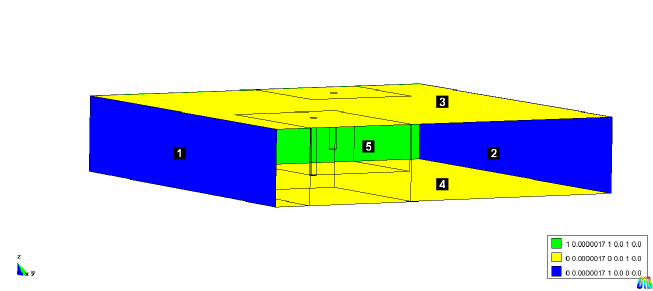
\includegraphics[scale=0.75]{img/datos_condiciones_ransol_fijar_velocidadinterno_leyendas}}
\caption{Velocidades Fijas}
\label{datos_condiciones_ransol_fijar_velocidadinterno_leyendas}
\end{figure}
%%%%%%%%%%%%%%%%%%%%%%%%%%%%%%
\subsubsection*{Fijar Velocidad}
Como se puede ver en la figura (\ref{datos_condiciones_ransol_fijar_velocidadinterno_leyendas}) las condiciones asignadas a cada una de las superficies enumeradas son las siguientes:

\begin{enumerate}

\item Superficie 1 y 2:

\begin{eqnarray*}
V_x&=&0.0000017~[m/s]\\
Fija~V_y&=&0.0~[m/s]\\
V_z&=&0.0~[m/s]
\end{eqnarray*}
Observar, que en las superficies 1 y 2 marcadas en la figura (\ref{datos_condiciones_ransol_fijar_velocidadinterno_leyendas}) se fija la velocidad $V_y$ a $0$, esto se hace con el objetivo de impedir que el fluido escape del dominio (impermeabilidad de las paredes laterales). En la dirección de $x$ y $y$ el movimiento es libre.

\item Superficie 3 y 4:

\begin{eqnarray*}
V_x&=&0.0000017~[m/s]\\
V_y&=&0.0~[m/s]\\
Fija~V_z&=&0.0~[m/s]
\end{eqnarray*}

En estas superficies se fija la velocidad $V_z$ a $0$. En la superficie marcada con el número 4 en la figura (\ref{datos_condiciones_ransol_fijar_velocidadinterno_leyendas}), se lo hace para representar la impermeabilidad de la superficie inferior del campo, por otro lado en la superficie marcada con 3, representa la no existencia de recarga sobre el campo. En las direcciones de $x$ y $y$ el movimiento es libre.

\item Superficie 5:

\begin{eqnarray*}
Fija~V_x&=&0.0000017~[m/s]\\
Fija~V_y&=&0.0~[m/s]\\
Fija~V_z&=&0.0~[m/s]\\
\end{eqnarray*}

Se puede observar que en esta superficie, se fijan las velocidades en las 3 direcciones, $x$, $y$ y $z$. Esto modela la entrada de agua que se desplaza en una sola dirección ($x$). Además ese desplazamiento es a la misma velocidad con el que se determino la constante de permeabilidad $k$ de la \emph{Ley de Darcy}.

\end{enumerate}
%%%%%%%%%%%%%%%%%%%%%%%%%%%%%%
\subsubsection*{Fijar Presión}
En la figura \ref{datos_condiciones_ransol_presion} se puede observar que se fijó un valor de referencia para la presión en la superficie del extremo final de salida del campo con valor igual a $0.0~\left[Pa\right]$. Esto significa que los resultados que obtendremos para la presión serán relativos a esta condición.

\begin{figure}[tbhp]
\centerline{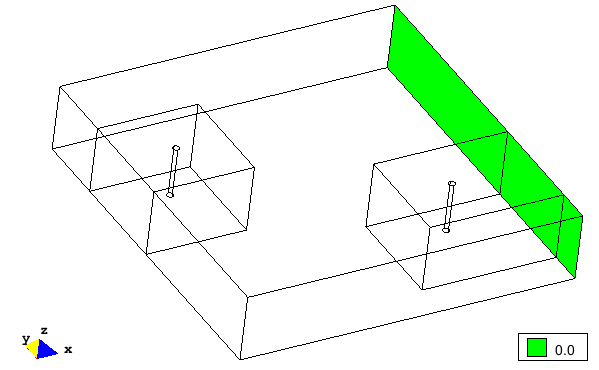
\includegraphics[scale=0.75]{img/datos_condiciones_ransol_presion}}
\caption{Condición fija de presión}
\label{datos_condiciones_ransol_presion}
\end{figure}
%%%%%%%%%%%%%%%%%%%%%%%%%%%%%%
\subsubsection*{Campo de Velocidad}
Para modelar la extracción de agua de los pozos, se aplicó un campo de velocidad como se observa en la figura (\ref{datos_condiciones_ransol_campo_de_velocidad}).
Para ambos pozos se genero una función dependiente del tiempo que modela el proceso de extracción de agua de la bomba durante un periodo de tiempo. En las figuras (\ref{grafica1_0085}) y (\ref{grafica1_0057}) se puede observar una pendiente creciente entre los pasos 100 y 500 (encendido de la bomba de extracción de agua) y una pendiente decreciente entre los pasos de tiempo 50000 y 50400 (apagado de la bomba de extracción de agua).
Entre los valores que se encuentran entre 500 y 50000 la velocidad es constante igual a la velocidad de extracción que posee la bomba del pozo.

A continuación se presentan las condiciones asignadas a cada pozo:
\begin{itemize}
\item Pozo 1: 
\begin{eqnarray} \label{pozo1_funcion}
\nonumber
Fijar~ValorX&=&0.0~[m/s]\\
\nonumber
Fijar~ValorY&=&0.0~[m/s]\\
Fijar~ValorZ&=& if(t<=100 | t>50400)then(vz=0)else(if(t>100 \& t<=500)then\\
\nonumber
&&(vz=0.00021*(t-100))else(if(t>500 \& t<=50000)then(vz=0.085)\\&&
\nonumber
else(vz=-0.00021*(t-50400))endif)endif)endif~~[m/s]
\end{eqnarray}
La función escrita para el $ValorZ$ en (\ref{pozo1_funcion}) se puede observar en la figura (\ref{grafica1_0085}) y viene dada por la función matemática (\ref{vz_ecuacion_pozo1})

%
\begin{equation}\label{vz_ecuacion_pozo1}
Vz_1(t) = \left\{
\begin{array}{l@{,\quad}l}
0 & t\leqslant 100 \vee t > 50400 \\
0.00021*(t-100) & t > 100 \wedge t\leqslant 500 \\
0.085 & t > 500 \wedge t\leqslant 50000 \\
-0.00021*(t-50400) & eoc
\end{array}
\right.
\end{equation}
%

\begin{figure}[tbhp]
\centerline{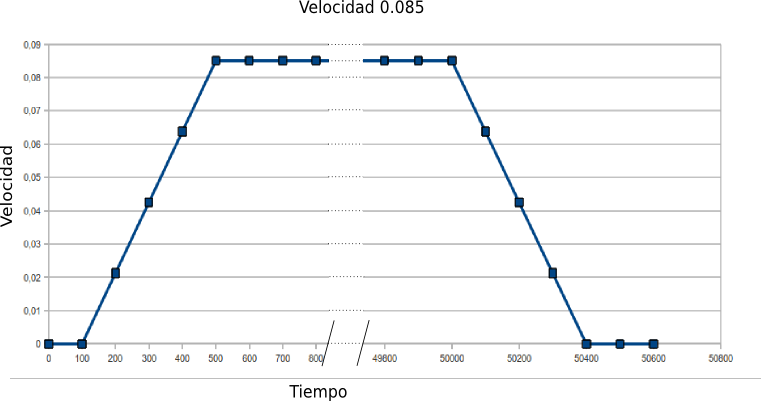
\includegraphics[scale=0.3]{graficas/0085}}
\caption{Función tiempo vs. velocidad de campo de velocidad en Z representada en (\ref{pozo1_funcion}) y (\ref{vz_ecuacion_pozo1})}
\label{grafica1_0085}
\end{figure}

\item Pozo 2:
\begin{eqnarray} \label{pozo2_funcion}
\nonumber
Fijar~ValorX&=&0.0~[m/s]\\
\nonumber
Fijar~ValorY&=&0.0~[m/s]\\
Fijar~ValorZ&=& if(t<=100 | t>50400) then(vz=0)else(if(t>100 \& t<=500)then\\
\nonumber
&&(vz=0.00014*(t-100))else(if(t>500 \& t<=50000)then(vz=0.057)\\&&
\nonumber
else(vz=-0.00014*(t-50400))endif)endif)endif~~[m/s]
\end{eqnarray}
La función escrita para el $ValorZ$ en (\ref{pozo2_funcion}) se puede observar en la figura (\ref{grafica1_0057})  y viene dada por la función matemática (\ref{vz_ecuacion_pozo2})
%
\begin{equation}\label{vz_ecuacion_pozo2}
Vz_2(t) = \left\{
\begin{array}{l@{,\quad}l}
0 & t \leqslant 100\vee t > 50400 \\
0.00014*(t-100) & t > 100 \wedge t \leqslant 500 \\
0.057 & t > 500 \wedge t \leqslant 50000 \\
-0.00014*(t-50400) & eoc
\end{array}
\right.
\end{equation}
%

\begin{figure}[tbhp]
\centerline{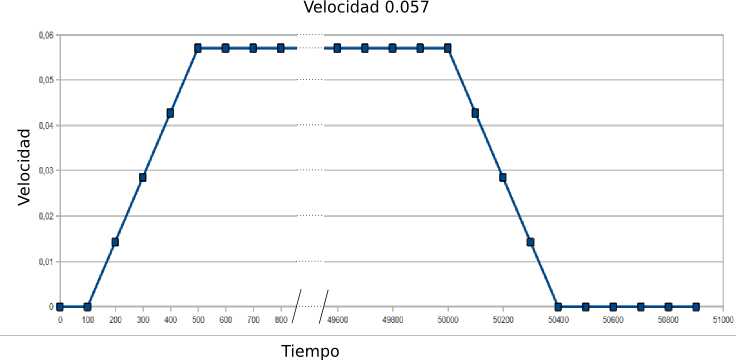
\includegraphics[scale=0.3]{graficas/0057}}
\caption{Función tiempo vs. velocidad de campo de velocidad en Z representada en (\ref{pozo2_funcion}) y (\ref{vz_ecuacion_pozo2})}
\label{grafica1_0057}
\end{figure}

\end{itemize}
\begin{figure}[tbhp]
\centerline{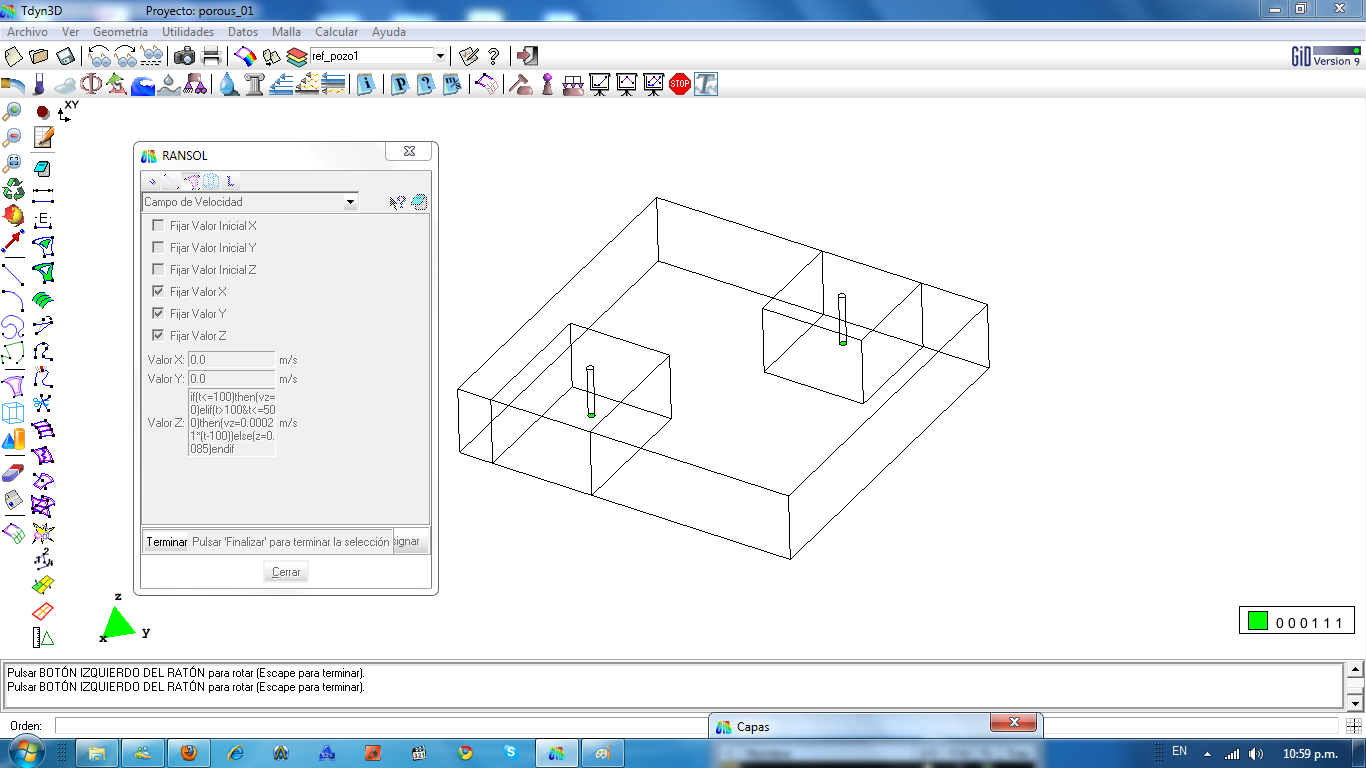
\includegraphics[scale=0.75]{img/datos_condiciones_ransol_campo_de_velocidad}}
\caption{Condición de campo de velocidades}
\label{datos_condiciones_ransol_campo_de_velocidad}
\end{figure}
%%%%%%%%%%%%%%%%%%%%%%%%%%%%%%%%%%%%%%%%%%%%%%%%%%%%%%%%%%%%%%%%%%%%%%%%%%%%%%%%%%%%%%%%%%%%%%%%%%%
\subsection{Mallado}
Para el mallado, se asignaron diferentes tamaños a las superficies debido a que se deseó obtener un mayor detalle en las cercanías de ambos pozos. Para ello se subdividió el dominio como se muestra en las figuras \ref{cotas_superiores_generalesXY} y \ref{cotas_superiores_detallesXY}, luego se aplicó una malla no estructurada de diferentes tamaños para las diferentes entidades como se puede ver en las figuras \ref{tam_malla_xy} y \ref{tam_malla_pozo_interior}. Además, en las preferencias de mallado de Gid (Utilidades $\rightarrow$ preferencias $\rightarrow$ pestaña malla), se fijó la transición de tamaños no estructurados a $0.4$.
A continuación, se presentan los tipos y cantidades de elementos con los que esta conformado la geometría:
\begin{itemize}
\item Número de nodos: 118551
\item Número de tetraedros: 651913. En la Fig. \ref{calidadtetraedros} se puede observar la calidad del mallado.
\item Número de triángulos: 43082. En la Fig. \ref{calidadtriangulos} se puede observar la calidad del mallado.
\item Total de elementos: 694995
\end{itemize}

\begin{figure}[tbhp]
\centerline{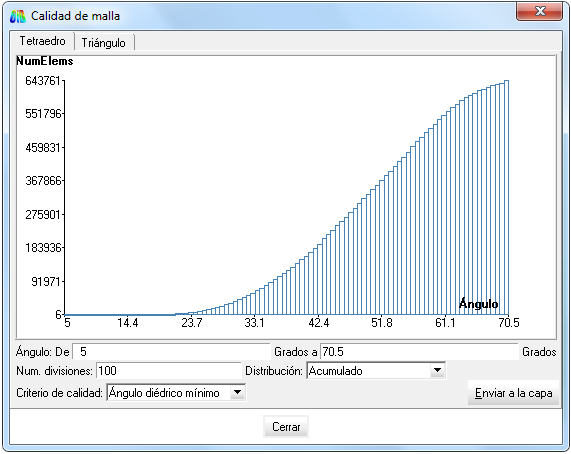
\includegraphics[scale=0.60]{img/cant_tetraedros}}
\caption{Calidad de la Malla - Tetraedros}
\label{calidadtetraedros}
\end{figure}

\begin{figure}[tbhp]
\centerline{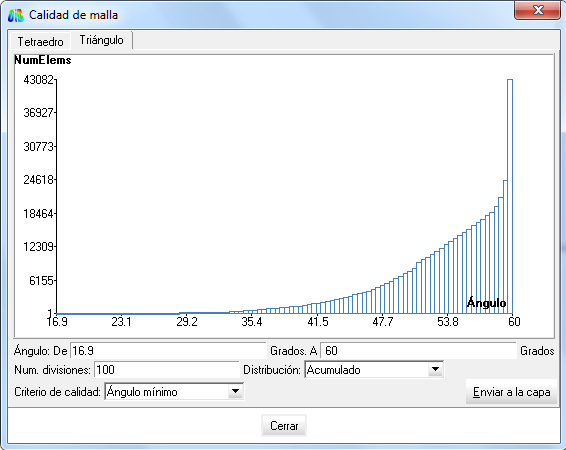
\includegraphics[scale=0.60]{img/cant_triangulos}}
\caption{Calida de la Malla - Triángulos}
\label{calidadtriangulos}
\end{figure}

\begin{figure}[tbhp]
\centerline{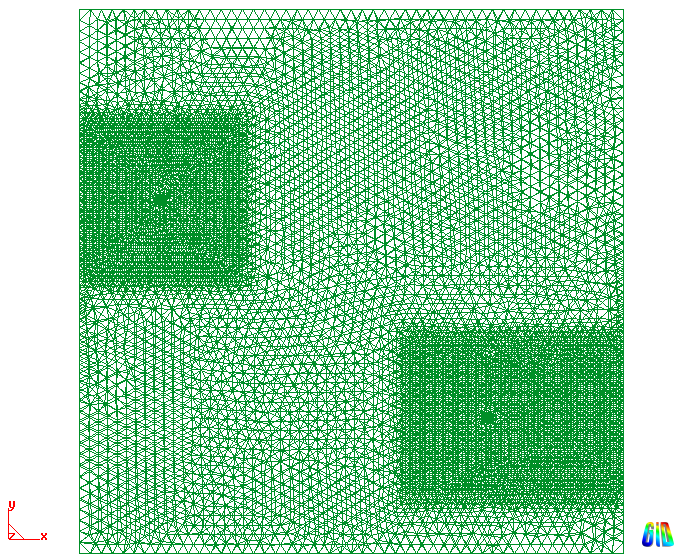
\includegraphics[scale=0.75]{img/contorno_malla_xy}}
\caption{Vista en el plano XY de la malla}
\label{contorno_malla_xy}
\end{figure}

%\begin{figure}[tbhp]
%\centerline{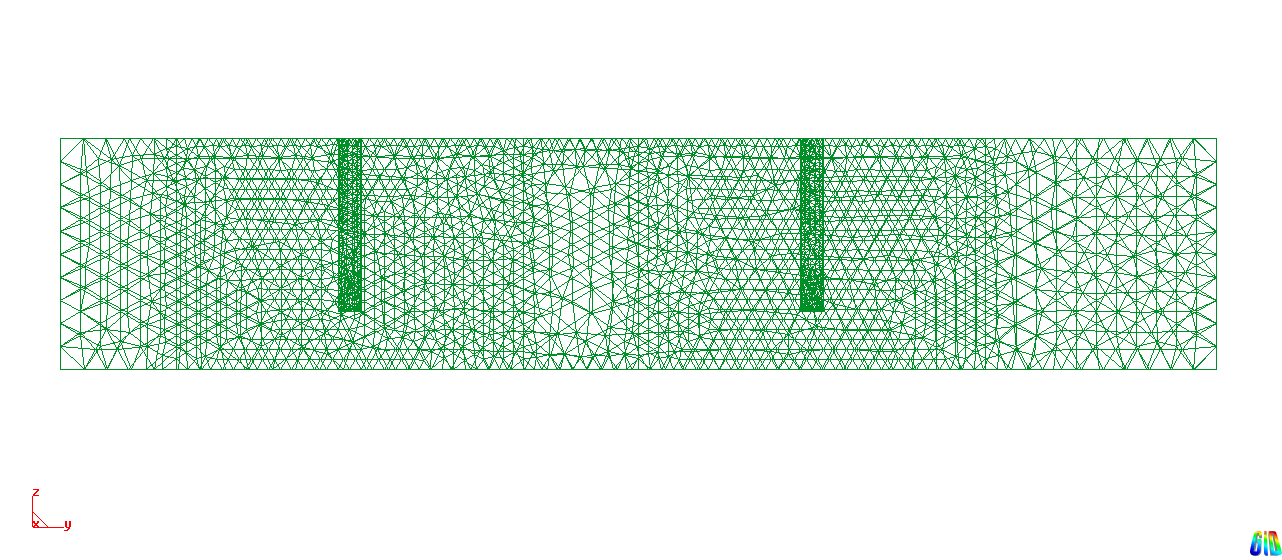
\includegraphics[scale=0.50]{img/contorno_malla_yz}}
%\caption{Vista en el plano YZ de la malla}
%\label{contorno_malla_yz}
%\end{figure}

\begin{figure}[tbhp]
\centerline{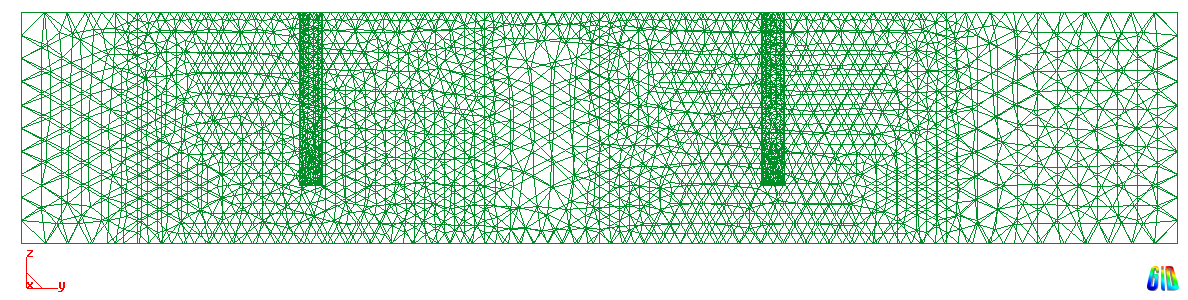
\includegraphics[scale=0.50]{img/contorno_malla_yz1}}
\caption{Vista en el plano YZ de la malla}
\label{contorno_malla_yz1}
\end{figure}

\begin{figure}[tbhp]
\centerline{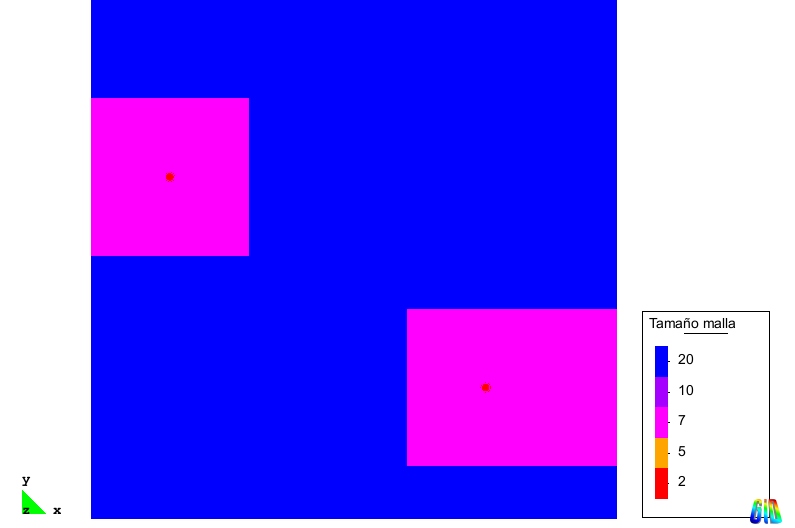
\includegraphics[scale=0.50]{img/tam_malla_xy}}
\caption{Tamaños de elementos de la malla - Vista en el plano XY}
\label{tam_malla_xy}
\end{figure}

\begin{figure}[tbhp]
\centerline{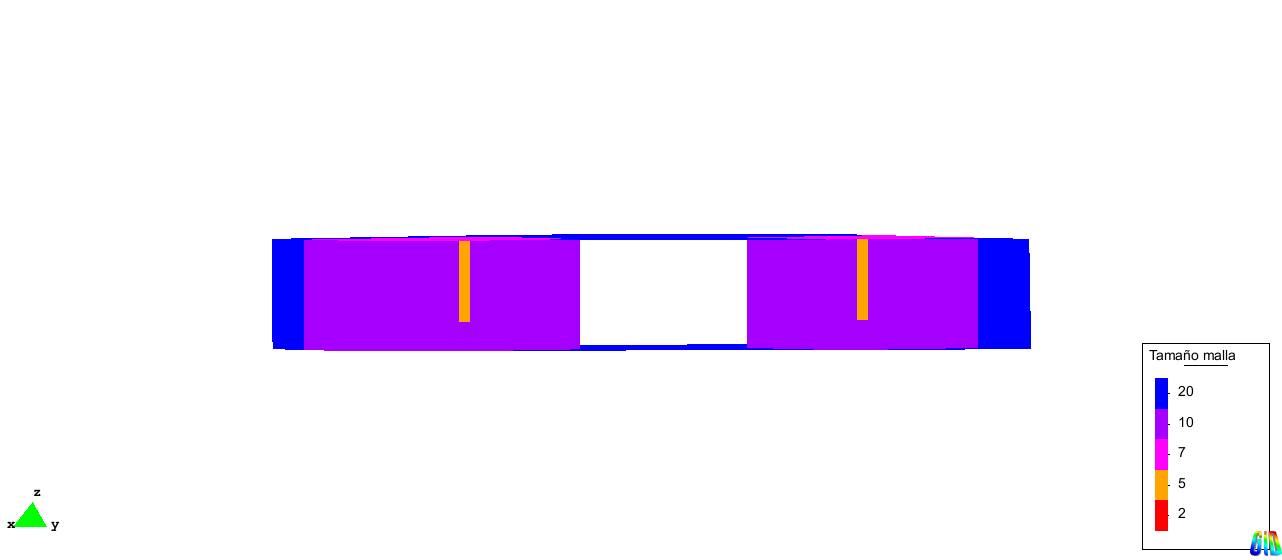
\includegraphics[scale=0.50]{img/tam_malla_pozo_interior}}
\caption{Tamaños de elementos de la malla - Corte transversal}
\label{tam_malla_pozo_interior}
\end{figure}
%%%%%%%%%%%%%%%%%%%%%%%%%%%%%%%%%%%%%%%%%%%%%%%%%%%%%%%%%%%%%%%%%%%%%%%%%%%%%%%%%%%%%%%%%%%%%%%%%%%
\subsection{Condiciones temporales}
La simulación se llevo a cabo con un $\Delta t = 100 \left[s\right]$ y se simularon 50400 o 50500 pasos \begin{Large}
ver!\\
\end{Large}
%
%%%%%%%%%%%%%%%%%%%%%%%%%%%%%%%%%%%%%%%%%%%%%%%%%%%%%%%%%%%%%%%%%%%%%%%%%%%%%%%%%%%%%%%%%%%%%%%%%%%
\subsection{Ejecución}
cambiar el titulo esto es como se llevo a cabao la corrida
ver graficos en un nodo o punto la evolucion de una variable. -> point evolution ->velocity->module->elijo un nodo
%%%%%%%%%%%%%%%%%%%%%%%%%%%%%%%%%%%%%%%%%%%%%%%%%%%%%%%%%%%%%%%%%%%%%%%%%%%%%%%%%%%%%%%%%%%%%%%%%%
%%%%%%%%%%%%%%%%%%%%%%%%%%%%%%%%%%%%%%%%%%%%%%%%%%%%%%%%%%%%%%%%%%%%%%%%%%%%%%%%%%%%%%%%%%%%%%%%%%
%%%%%%%%%%%%%%%%%%%%%%%%%%%%%%%%%%%%%%%%%%%%%%%%%%%%%%%%%%%%%%%%%%%%%%%%%%%%%%%%%%%%%%%%%%%%%%%%%%
\section{Resultados}
v(veloc) -> lineas de flujo/vect
p->equipotenciales
realizar cortes
lo que vamos a ver va a ser las equipotenciales (lineas de presion que son perpendiculares al flujo).siempre es contraria a la linea de velocidad\\
En los softwares específicos de hidrogeología, fijate que aca tenes el esquema de calculo que es una malla muy guresa en dos dimensiones, que te va a dar isocurvas de niveles. Se va a ver como esto va bombeando y ese nivel de agua cerca de la bomba va ir deprimiendose formando el cono de desenso. Eso, asi de esa forma aca no lo vamos a poder hacer, porque para poder hacer eso en 3D (en 2D si se puede) tenes que tener un soft que distinga entre suelo no saturado y suelo saturado. En el suelo saturado las ecs de gobierno son distintas a las del no saturado. El soft que tenemos solamente tiene las ecs de gob del suelo saturado, el no saturado tiene un modelo mucho mas complejo, en realidad estos modelos son bidimensionales porque no calculan el flujo en suelo saturado, lo que calculan seria la curva, la interfaz, seria la sup que los separa, nada mas, sería la ubicación de esa sup que distingue zona saturada de la no saturada. que tiene ecuaciones simples, pero no calcula detalles del flujo, este modelo calcula el flujo en suelo saturado. 
Se coincidiera que se esta en presencia de un estrato de suleo saturado (esto es saturado de agua). 
Vamos a tener lineas equipotenciales (unen lineas de igual potencial hidráulico) las cuales son perpendiculares a las lineas del flujo y serian valores de presión que ejerce el agua sobre el suelo. Esas líneas equipotenciales van a ser equivalentes en interpretación a las lineas de superficie que se calculan tradicionalmente en hidrologia.
%%%%%%%%%%%%%%%%%%%%%%%%%%%%%%%%%%%%%%%%%%%%%%%%%%%%%%%%%%%%%%%%%%%%%%%%%%%%%%%%%%%%%%%%%%%%%%%%%%
%%%%%%%%%%%%%%%%%%%%%%%%%%%%%%%%%%%%%%%%%%%%%%%%%%%%%%%%%%%%%%%%%%%%%%%%%%%%%%%%%%%%%%%%%%%%%%%%%%
%%%%%%%%%%%%%%%%%%%%%%%%%%%%%%%%%%%%%%%%%%%%%%%%%%%%%%%%%%%%%%%%%%%%%%%%%%%%%%%%%%%%%%%%%%%%%%%%%%
\section{Conclusiones}
si el mod respondio
que problemas tuvimos? ahi hacer mencion al pozo grande y tiempo de calculo...
pozo real vs pozo simulado
%%%%%%%%%%%%%%%%%%%%%%%%%%%%%%%%%%%%%%%%%%%%%%%%%
%%%%%%%%%%%%%%%%%%%%%%%%%%%%%%%%%%%%%%%%%%%%%%%%%
%%%%%%%%%%%%%%%%%%%%%%%%%%%%%%%%%%%%%%%%%%%%%%%%%
\end{document}